%   ##
%
%   Band VIII, 3 N.~??A07
%   Signatur/Tex-Datei: LH_37_01_022-023
%   RK-Nr. 38538
%   Überschrift: De vibrationibus aeris tensi
%   Datierung: [??August 1682 -- erste Hälfte 1684??]
%   WZ: (keins)
%.  SZ: (keins)
%.  Bilddateien (PDF): LH_37_01_022-023_d1; LH_37_01_022-023_d2; LH_37_01_022-023_d3; LH_37_01_022-023_d4; LH_37_01_022-023_d5 (insgesamt fünf)
%
%
\begin{ledgroupsized}[r]{120mm}
\footnotesize
\pstart
\noindent\textbf{Überlieferung:}
\pend
\end{ledgroupsized}
\begin{ledgroupsized}[r]{114mm}
\footnotesize
\pstart \parindent -6mm
\makebox[6mm][l]{\textit{L}}%
Konzept: LH~XXXVII~1 Bl.~22\textendash23.
Ein Bogen~4\textsuperscript{o}.
Dreieinhalb voll beschriebene Seiten;
die untere Hälfte von Bl.~23~v\textsuperscript{o} ist leer.
% Keine Wasserzeichen.
\pend
\end{ledgroupsized}
%
\begin{ledgroupsized}[r]{114mm}
\footnotesize%
\pstart%
\parindent -6mm
\makebox[6mm][l]{\textit{E}}%
\textsc{Gerland} 1906, S.~31\textendash35.\cite{00197}
\pend%
\end{ledgroupsized}
%
\vspace*{5mm}
\begin{ledgroup}
\footnotesize
\pstart
\noindent
\textbf{Datierungsgründe:}
Der vorliegende Entwurf N.~21 ist dem Ansatz nach eine Untersuchung darüber, ob die Schwingungen einer Luftmasse ebenso isochron sind wie die einer gezupften Saite.
Ausschlaggebend für die Datierung ist die Ausgangshypothese der Untersuchung (siehe S.~\refpassage{LH_37_01_022r_grundhypothese_ihutd-1}{LH_37_01_022r_grundhypothese_ihutd-2} samt Diagramm \lbrack\textit{Fig.~1}\rbrack):
An den Spannungszuständen einer Luftmasse in einem verschlossenen Behälter lasse sich allgemein zeigen, dass die Dehnung eines elastischen Körpers in direktem Verhältnis zur angewandten Spannkraft stehe (wie dies etwa auch bei einer Saite oder einem Seil der Fall ist).
An diese Hypothese knüpft Leibniz auch in den Entwürfen N.~14\textsubscript{3} (S.~\refpassage{LH_35_09_16_020v_kolbenmodell-1}{LH_35_09_16_020v_kolbenmodell-2} samt \lbrack\textit{Fig.~5}\rbrack) und N.~14\textsubscript{7} (S.~\refpassage{LH_35_09_16_002_Beweis-1}{LH_35_09_16_002_Beweis-2} samt \lbrack\textit{Fig.~2}\rbrack) sowie in dem verwandten Brief an E.~Mariotte von März/April 1683 (\protect\index{Namensregister}{\textso{Mariotte}, Edme, Seigneur de Chazeuil ca. 1620\textendash1684}\cite{01262}\textit{LSB} III,~3 N.~456, S.~795.21\textendash796.3) an, am ausführlichsten wohl aber im Entwurf LH~XXXVII~3 Bl.~125\textendash127 (welcher voraussichtlich in einem künftigen Band von \textit{LSB} VIII ediert wird).
Während die Entstehungszeit von LH~XXXVII~3 Bl.~125\textendash127 noch nicht ermittelt ist, lassen sich die Entwürfe N.~14\textsubscript{3} und N.~14\textsubscript{7} insgesamt auf die Zeitspanne zwischen Ende Januar 1683 und der ersten Hälfte 1684 datieren (siehe die editorische Vorbemerkung zum Textkomplex N.~14, S.~\refpassage{AE_1684_319-325_intro_LeibizAnMariotte-1}{AE_1684_319-325_intro_LeibizAnMariotte-1}\,ff.).
Ein ähnlicher Ansatz wie in N.~21 findet sich zwar auch in früheren Texten vom Dezember 1674 (etwa \textit{LSB} VIII,~1 N.~54)
und im Wesentlichen in der Aufzeichnung N.~7 (S.~\refpassage{LH_35_09_15_022v_Beweis_sgtk-1}{LH_35_09_15_022v_Beweis_sgtk-2});
eine Entstehung vor dem Herbst 1675 ist im Fall von N.~21 aber schon aufgrund der verwendeten mathematischen Notation unmöglich,
während der in N.~21 verwendete Kraftbegriff eine Entstehung vor Anfang 1678 ausschließt.
Der ausschlaggebende Bezug auf den Isochronimsus schwingender Saiten ist vielmehr Grund für die Annahme, dass N.~21 erst nach den Texten N.~8, 9 und 10 (Dezember 1680/Anfang 1681) entstand, in denen diese Thematik ausführlich behandelt wird.
Aber insbesondere der inhaltliche Zusammenhang mit N.~14\textsubscript{3} und N.~14\textsubscript{7} lässt vermuten, dass N.~21 nicht wesentlich früher entstanden war.
Daraus ergibt sich der am meisten wahrscheinliche Terminus post quem der Datierung.
Diese Vermutung wird dadurch gestützt, dass Leibniz sich zu etwa der gleichen Zeit noch mit dem Phänomen der Schallausbreitung befasste, welches er eben auf die in N.~21 thematisierten Schwingungen der Luft als elastischen Mediums zurückführte (siehe den zwischen der zweiten Hälfte August 1681 und der ersten Hälfte 1685 entstandenen Textkomplex N.~12 und die editorische Vorbemerkung hierzu).
\pend%
\pstart%
Andererseits weist der Entwurf N.~21 auch eine bemerkenswerte inhaltliche Verwandtschaft mit Untersuchungen über die elastische Kraft der Luft aus den späten Achtziger Jahren auf: insbesondere mit N.~27\textsubscript{1} (Juli 1686) und N.~27\textsubscript{2} (27. August 1689).
Beide letztere Texte stellen gleichsam eine Fortsetzung der Ausführungen am Schluss von N.~21 (bes. S.~\refpassage{LH_37_01_023v_Schluss_girt-1}{LH_37_01_023v_Schluss_girt-2}) dar, wobei N.~27\textsubscript{2} aber ausdrücklich von N.~27\textsubscript{1} herrührt (siehe die editorische Vorbemerkung zum Textkomplex N.~27, S.~\pageref{LH_35_10_08_010-011+LH_35_10_08_015_Vorbemerkung}).
Anhand der inhaltlichen Verwandtschaft zwischen N.~21 und N.~27 und angesichts der Abhängigkeitsverhältnisse zwischen N.~27\textsubscript{1} und N.~27\textsubscript{2} erweist sich für N.~21 eine Entstehungszeit bis Juli 1686 als plausibel.
Daraus ergibt sich die für N.~21 vorgeschlagene Gesamtdatierung.
Eine etwas frühere (ab 1681?) oder spätere (bis August 1689?) Datierung ist allerdings nicht auszuschließen.

% ((??Inhaltliche Übereinstimmung mit ??A02, ??A03 und ??A04. Deshalb vorgeschlagene Datierung ist: ??Anfang 1681 bis ??zweite Hälfte 1684. Ausschlaggebend könnte die Übereinstimmung mit ??A04 sein. Dann wäre möglich, die Datierung auf ??Anfang 1682 bis ??zweite Hälfte 1684 einzugrenzen, vielleicht noch genauer. Auf eine konkrete Stelle hinweisen, an der die Übereinstimmung deutlich wird. Datierung bleibt hypothetisch/relativ. [[RK: Komplex Math. Schr. 1684]]??))\\
\pend
\end{ledgroup}
%
% \vspace*{8mm}
\newpage%
%
%
\count\Bfootins=1000
\count\Afootins=1200
\count\Cfootins=1000
%
%
\pstart%
\normalsize%
\noindent%
\lbrack22~r\textsuperscript{o}\rbrack\
\pend%
% Überschrift
\pstart%
\centering%
De Vibrationibus aeris tensi\protect\index{Sachverzeichnis}{vibratio aeris}\protect\index{Sachverzeichnis}{aer tensus}
\pend%
\vspace{0.5em}%
%
\pstart%
\noindent%
Fingamus\edlabel{LH_37_01_022r_grundhypothese_ihutd-1}
\edtext{Embolum\protect\index{Sachverzeichnis}{embolus}
exacte respondentem Tubo\protect\index{Sachverzeichnis}{tubus}
vas\protect\index{Sachverzeichnis}{vas aere plenum}
Aere communi\protect\index{Sachverzeichnis}{aer communis}
(\protect\vphantom)%
hoc est neque compresso\protect\index{Sachverzeichnis}{aer compressus}
ultra statum\protect\index{Sachverzeichnis}{status}
reliqui aeris ambientis,\protect\index{Sachverzeichnis}{aer ambiens}
neque dilatato\protect\index{Sachverzeichnis}{aer dilatatus}%
\protect\vphantom()
plenum ingredienti,
nonnihil extrahi ex tubo,\protect\index{Sachverzeichnis}{tubus}}{%
\lemma{Embolum}\Bfootnote{%
\textit{(1)}~ex
\textit{(2)}~in
\textit{(3)}~exacte respondentem % Tubo vas 
\lbrack...\rbrack\ Aere communi
\textit{(a)}~plenum
\textit{(b)}~(\protect\vphantom)hoc est \lbrack...\rbrack\ dilatato\protect\vphantom() plenum
\textit{(aa)}~nonnihil
\textit{(bb)}~ingredienti, nonnihil
\textit{(aaa)}~inde
\textit{(bbb)}~extrahi ex tubo,%
~\textit{L}}}
ut ita aer dilatetur,
deinde antequam totus
\edtext{egrediatur, a trahente subito dimitti;
manifestum est non sine vi\protect\index{Sachverzeichnis}{vis} rursus}{%
\lemma{egrediatur,}\Bfootnote{%
\textit{(1)}~et a po
\textit{(2)}~rurs
\textit{(3)}~a trahente \lbrack...\rbrack\ manifestum est
\textit{(a)}~magna vi
\textit{(b)}~non sine
\textit{(aa)}~impetu
\textit{(bb)}~vi rursus%
~\textit{L}}}
in tubum\protect\index{Sachverzeichnis}{tubus} subingredi debere,
nec tantum in priorem statum\protect\index{Sachverzeichnis}{status} redire,
sed impetu concepto\protect\index{Sachverzeichnis}{impetus conceptus} ultra provehi,
aeremque inclusum\protect\index{Sachverzeichnis}{aer inclusus} comprimere;
moxque ab eo rursus repulsum impetu concepto\protect\index{Sachverzeichnis}{impetus conceptus} contrario iterum
\edtext{ultra justam}{%
\lemma{ultra}\Bfootnote{%
\textit{(1)}~mediam
\textit{(2)}~justam%
~\textit{L}}}
mensuram exire,
et nova dilatatione\protect\index{Sachverzeichnis}{dilatatio} facta
\edtext{denuo deinde}{%
\lemma{denuo}\Bfootnote{%
\textit{(1)}~mox
\textit{(2)}~deinde%
~\textit{L}}}
intra tubum\protect\index{Sachverzeichnis}{tubus}
\edtext{compelli, easque vibrationes\protect\index{Sachverzeichnis}{vibratio} aliquoties reciprocare.}{%
\lemma{compelli,}\Bfootnote{%
\textit{(1)}~eamque
\textit{(2)}~easque
\textbar~reciprocationes\protect\index{Sachverzeichnis}{reciprocatio} sive \textit{gestr.}~%
\textbar\ vibrationes aliquoties reciprocare.%
~\textit{L}}}
Jam investigare operae pretium est,
an tempora\protect\index{Sachverzeichnis}{tempus vibrationis}
\edtext{vibrationum
\lbrack emboli\protect\index{Sachverzeichnis}{embolus}\rbrack\
magis vel minus extracti sint aequalia,}{%
\lemma{vibrationum}\Bfootnote{%
\textit{(1)}~sint ae
\textit{(2)}~majorum et minorum
\textit{(3)}~\textbar~tubi\protect\index{Sachverzeichnis}{tubus} \textit{ändert Hrsg.}~%
\textbar\ magis \lbrack...\rbrack\ sint aequalia,%
~\textit{L}}}
\edtext{quemadmodum
\edtext{sic satis}{%
\lemma{sic}\Bfootnote{% \hspace*{-0,5mm}
satis \textit{erg.~L}}}
esse experimur in chordis pulsatis.\protect\index{Sachverzeichnis}{chorda pulsata}%
}{\lemma{quemadmodum \lbrack...\rbrack\ pulsatis}\Cfootnote{%
Den Iso\-chro\-nis\-mus der Schwingungen gespannter Saiten hatte Leibniz zunächst in Aufzeichnungen aus Dezember 1680/Anfang 1681 untersucht;
vgl.
N.~\ref{41152_5}, %??A10\textsubscript{5} 
S.~\refpassage{LH_35_09_15_015v_isochron-1}{LH_35_09_15_015v_isochron-2};
N.~\ref{41152_6}, %??A10\textsubscript{6} 
S.~\refpassage{LH_35_09_15_016r_propositio3-1}{LH_35_09_15_016r_propositio3-2};
N.~\ref{41153}, % ??A11 
S.~\refpassage{LH_35_09_15_003r_aequdiut-1}{LH_35_09_15_003v_aequdiut-2};
N.~\ref{41156}, %??A13 
S.~\refpassage{LH_35_09_15_021r_propositio1-1}{LH_35_09_15_021r_propositio1-2}.
Das Phänomen behandelte er wieder in späteren Entwürfen;
vgl.
N.~\ref{58256_1}; %??A34.1
N.~\ref{58256_2} %??A34.2
(August bis November 1689);
N.~\ref{RK60353}; %??A46
N.~\ref{RK60301}, %??A45 
bes. S.~\refpassage{LH_37_05_046r_Isochronismusbeweis-1}{LH_37_05_046r_Isochronismusbeweis-2}
(Mitte 1690 bis 1695).}}
\pend%
%
%  \newpage% REIN VORLÄUFIG !!!
%  \vspace*{0.0em}%
%  \centerline{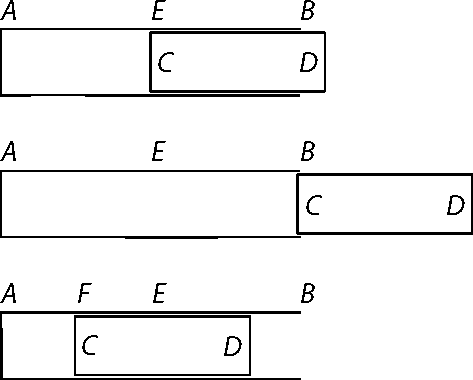
\includegraphics[width=0.42\textwidth]{gesamttex/edit_VIII,3/images/LH_37_01_022-023_d1.pdf}}%\\
%  \vspace*{1.0em}
%  \centerline{\lbrack\textit{Fig.~1}\rbrack}%
%  \edtext{}{\lemma{\lbrack\textit{Fig.~1}\rbrack}\killnumber\Cfootnote{***************************}}
%  \vspace*{1.5em}%
%
\pstart%
Concipiamus autem majoris facilitatis causa,
vas\protect\index{Sachverzeichnis}{vas} esse
\edtext{tubum}{%
\lemma{tubum}\Bfootnote{\textit{erg.~L}}}
cylindricum\protect\index{Sachverzeichnis}{tubus cylindricum}
\edtext{$AB;$}{%
\lemma{$AB$}\Bfootnote{%
~\textit{erg.~L}}}
\edtext{cujus pars}{%
\lemma{cujus}\Bfootnote{%
\hspace{-0,5mm}\textbar~media \textit{gestr.}~%
\textbar\ pars%
~\textit{L}}}
\edtext{$AE$}{%
\lemma{$AE$}\Bfootnote{\textit{erg.~L}}}
sit aere communi\protect\index{Sachverzeichnis}{aer communis} plena,
\edtext{altera pars}{%
\lemma{altera}\Bfootnote{%
\textit{(1)}~medietas
\textit{(2)}~pars%
~\textit{L}}}
\edtext{$EB$}{%
\lemma{$EB$}\Bfootnote{\textit{erg.~L}}}
embolo\protect\index{Sachverzeichnis}{embolus}
\edtext{$CD;$}{%
\lemma{$CD$}\Bfootnote{\textit{erg.~L}}}
embolum autem usque ad ostium\protect\index{Sachverzeichnis}{ostium} extrahi, non ultra,
ne pereat obturatio;\protect\index{Sachverzeichnis}{obturatio}
et jam videamus
\edtext{quid consequatur}{%
\lemma{quid}\Bfootnote{%\hspace*{-0,5mm}
\textbar~unde \textit{gestr.}~\textbar\ consequatur%
~\textit{L}}}
\edtext{si $C$ emboli extremitas transferatur}{%
\lemma{si}\Bfootnote{%
\textit{(1)}~embolus 
\textit{(a)}~ibi 
\textit{(b)}~a $C$ trans
\textit{(2)}~extremi
\textit{(3)}~$C$ emboli extremitas%
~\textit{L}}}
in $B,$
et ibi embolus\protect\index{Sachverzeichnis}{embolus} rursum
\edtext{dimittatur.
Quoniam}{%
\lemma{dimittatur.}\Bfootnote{%
\textit{(1)}~Ingredie
\textit{(2)}~Quoniam%
~\textit{L}}}
igitur effectus est aequalis suae causae,\protect\index{Sachverzeichnis}{aequipollentia causae et effectus}
embolus\protect\index{Sachverzeichnis}{embolus} rursum intromissus, non sistet in $E,$
sed introrsum progreditur usque in $F,$
donec vis compressionis,\protect\index{Sachverzeichnis}{vis compressionis}
\edtext{seu vis aeris}{%
\lemma{seu}\Bfootnote{%
\hspace{-0,5mm}vis
\textbar~elastica\protect\index{Sachverzeichnis}{vis elastica} \textit{gestr.}~%
\textbar\ aeris%
~\textit{L}}}
\edtext{compressi\protect\index{Sachverzeichnis}{aer compressus} $AFC,$}{%
\lemma{compressi}\Bfootnote{%
\textit{(1)}~$AF,$
\textit{(2)}~$AFC,$%
~\textit{L}}}
sit aequalis vi dilatationis\protect\index{Sachverzeichnis}{vis dilatationis}
seu vi aeris dilatati $ABC,$\protect\index{Sachverzeichnis}{aer dilatatus}
\edtext{\lbrack quod}{%
\lemma{\lbrack quod}%
\Cfootnote{Eckige Klammer von Leibniz.}}
\edtext{fiet
si ipsis $AB,$ $AE$ sit tertia proportionalis $AF,$%
}{%
\lemma{fiet}\Bfootnote{%
\textit{(1)}~si
\textit{(a)}~$AF$ \textbar~sit \textit{erg.}~\textbar\ te
\textit{(b)}~sit ipsis
\textit{(2)}~si ipsis % $AB,$ $AE$ sit tertia 
\lbrack...\rbrack\ proportionalis $AF,$%
~\textit{L}}} aere tantundem compresso\protect\index{Sachverzeichnis}{aer compressus} nunc,
quantum antea fuit
\edtext{dilatatus;\protect\index{Sachverzeichnis}{aer dilatatus} quos}{%
\lemma{dilatatus;}\Bfootnote{%
\textit{(1)}~quae
\textit{(2)}~quos%
~\textit{L}}}
duos status\protect\index{Sachverzeichnis}{status} inter se
aequilibrium\protect\index{Sachverzeichnis}{aequilibrium} facere,
seu aequales
\edtext{esse
\edtext{ostendemus.\rbrack}{%
\lemma{ostendemus.\rbrack}%
\Cfootnote{Eckige Klammer von Leibniz. Das Ergebnis der Untersuchung wird am Schluss (S.~\refpassage{LH_37_01_023v_Schluss_girt-1}{LH_37_01_023v_Schluss_girt-2}) zusammengefasst.}}
Extracto}{%
\lemma{esse}\Bfootnote{%
\hspace{-0,5mm}\textbar~sic \textit{gestr.}~%
\textbar\ ostendemus.\rbrack\
\textit{(1)}~Fingamus contingere sane operationem\protect\index{Sachverzeichnis}{operatio} in camera aliqua accurate clausa,\protect\index{Sachverzeichnis}{camera clausa} manifestum est
\textit{(2)}~Extracto%
~\textit{L}}}
embolo\protect\index{Sachverzeichnis}{embolus} ex $CE$ in $CB,$
columna aeris\protect\index{Sachverzeichnis}{columna aeris} aeque ampla elevata est
ad altitudinem $EB,$\protect\index{Sachverzeichnis}{altitudo lapsus}
\edtext{vel quod}{%
\lemma{vel}\Bfootnote{%
\textit{(1)}~quid
\textit{(2)}~quod%
~\textit{L}}}
idem est pondus $CD,$\protect\index{Sachverzeichnis}{pondus descendens}
quod ponamus huic columnae aequale,
fingendo tubum\protect\index{Sachverzeichnis}{tubus} esse ad horizontem
\edtext{erectum et pro columna aeris\protect\index{Sachverzeichnis}{columna aeris}
esse in vacuo;\protect\index{Sachverzeichnis}{vacuum}
porro punctum $F$}{%
\lemma{erectum}\Bfootnote{%
\textit{(1)}~; porro
\textit{(a)}~$F$
\textit{(b)}~punctum $F$
\textit{(2)}~et pro \lbrack...\rbrack\ punctum $F$%
~\textit{L}}}
tale esse debet,
\edtext{ut eo}{%
\lemma{ut}\Bfootnote{% \hspace*{-0,5mm}
\textbar~ab \textit{gestr.}~\textbar\ eo%
~\textit{L}}}
repulsum pondus $CD,$\protect\index{Sachverzeichnis}{pondus descendens}
rursus in $E$ praecise eam celeritatem\protect\index{Sachverzeichnis}{celeritas} acquirat,
quam ibi habebat,
cum introrsum
\edlabel{LH_37_01_022-023_d1_01}%
\edtext{}{{\xxref{LH_37_01_022-023_d1_01}{LH_37_01_022-023_d1_02}}{%
\lemma{pelleretur}\Bfootnote{%
\textit{(1)}~porro impulsu\protect\index{Sachverzeichnis}{impulsus}
\textit{(2)}~quomodo ut
\textit{(3)}~. Ut igitur motum omnem ponderis $C$ ingredientis
\textit{(4)}~. Ut igitur motum 
\textit{(a)}~accurate
\textit{(b)}~ponderis $C$ accurate%
~\textit{L}}}}%
pelleretur.\edlabel{LH_37_01_022r_grundhypothese_ihutd-2}
\pend
\pstart%
Ut igitur motum ponderis $C$\protect\index{Sachverzeichnis}{motus ponderis} accurate%
\edlabel{LH_37_01_022-023_d1_02}
cognoscamus\lbrack,\rbrack\
considerandum
\edtext{est gradus celeritatis\protect\index{Sachverzeichnis}{gradus celeritatis}}{%
\lemma{est}\Bfootnote{%
\textit{(1)}~impetus\protect\index{Sachverzeichnis}{impetus}
\textit{(2)}~gradus celeritatis%
~\textit{L}}}
\edtext{novos
qui ponderi $C$ cadenti\protect\index{Sachverzeichnis}{pondus cadens} imprimuntur
eo esse minores,
quo magis}{%
\lemma{novos}\Bfootnote{%
\textit{(1)}~semper esse eo minores, quo
\textit{(2)}~qui ponderi \lbrack...\rbrack\ minores, quo
\textit{(a)}~majo
\textit{(b)}~magis%
~\textit{L}}}
ingreditur embolus\protect\index{Sachverzeichnis}{embolus} in tubum,\protect\index{Sachverzeichnis}{tubus}
et resistentias aeris,\protect\index{Sachverzeichnis}{resistentia aeris}
qui semper est compressus,\protect\index{Sachverzeichnis}{aer compressus}
esse ut compressiones,\protect\index{Sachverzeichnis}{compressio} hoc est reciproce ut spatia.
\edtext{Nam aer\protect\index{Sachverzeichnis}{aer dilatatus}
cum dilatatus dicitur nostri respectu,
revera}{%
\lemma{Nam}\Bfootnote{%
\textit{(1)}~revera
\textit{(2)}~aer cum \lbrack...\rbrack\ respectu, revera%
~\textit{L}}} tantum
\pend%
%  \newpage% REIN VORLÄUFIG !!!
  \vspace{2.5em}%
  \centerline{\hspace*{-75mm}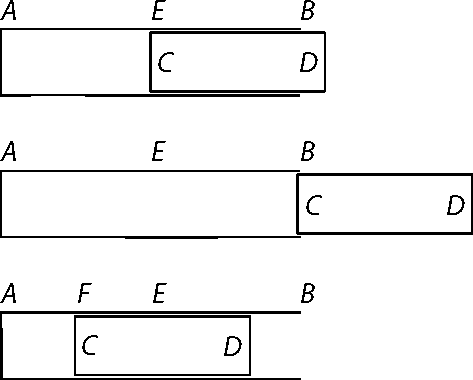
\includegraphics[width=0.44\textwidth]{gesamttex/edit_VIII,3/images/LH_37_01_022-023_d1.pdf}}%
  \vspace{1.0em}
  \centerline{\hspace*{-72mm}\lbrack\textit{Fig.~1}\rbrack}%
%  \vspace*{1.5em}%
  %
%
  \vspace*{-14.65em}%
  \centerline{\hspace*{38mm}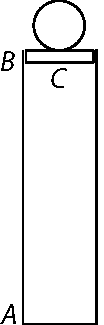
\includegraphics[width=0.10\textwidth]{gesamttex/edit_VIII,3/images/LH_37_01_022-023_d2.pdf}}%
  \vspace*{1.0em}
  \centerline{\hspace*{38mm}\lbrack\textit{Fig.~2}\rbrack}%
%  \newpage% REIN VORLÄUFIG !!!
%
%
  \vspace*{-12.8em}%
  \centerline{\hspace*{124mm}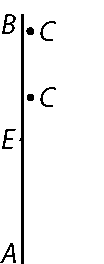
\includegraphics[width=0.103\textwidth]{gesamttex/edit_VIII,3/images/LH_37_01_022-023_d3.pdf}}%
  \vspace*{1.0em}
  \centerline{\hspace*{116mm}\lbrack\textit{Fig.~3}\rbrack}%
  %\vspace*{1.5em}%
%  \newpage
%
%
%
% \pstart% REIN VORLÄUFIG !!!
%
%   \vspace*{2.0em}% REIN VORLÄUFIG !!!
%   \hspace*{16mm}% REIN VORLÄUFIG !!!
%   \begin{minipage}[t]{0.30\textwidth}
%  \hspace*{-5mm}
%   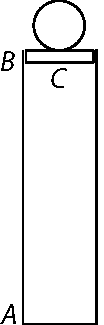
\includegraphics[width=0.30\textwidth]{gesamttex/edit_VIII,3/images/LH_37_01_022-023_d2.pdf}\\
%  \vspace*{2.0em}
%   \noindent\centering[\textit{Fig.~2}]
%   \end{minipage}
%
%   \hspace*{22mm}% Bitte mehr Abstand !!!
%   \begin{minipage}[t]{0.30\textwidth}
%  \hspace*{-5mm}
%   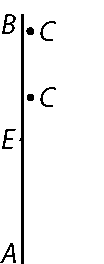
\includegraphics[width=0.30\textwidth]{gesamttex/edit_VIII,3/images/LH_37_01_022-023_d3.pdf}\\
%  \vspace*{2.0em}
%   \noindent\centering[\textit{Fig.~3}]
%   \end{minipage}
%
% \pend%
% \vspace*{2.0em}
%
%
\newpage
\pstart
\noindent
est minus compressus.\protect\index{Sachverzeichnis}{aer compressus}
Sit igitur
\edtext{$AB,$ $b,$ et}{%
\lemma{$AB,$}\Bfootnote{%
\hspace{-0,5mm}$b,$ et \textit{erg.~L}}}
\edtext{$AC$, $x$ varians}{%
\lemma{$AC$,}\Bfootnote{% \hspace*{-0,5mm}
$x$
\textit{(1)}~et
\textit{(2)}~varians%
~\textit{L}}}
%
\lbrack22~v\textsuperscript{o}\rbrack\ % Blatt 22v
%
pro vario situ\protect\index{Sachverzeichnis}{situs}
\edtext{ipsius $C;$ conatus}{%
\lemma{ipsius}\Bfootnote{%
\hspace{-0,5mm}$C;$
\textit{(1)}~impetus\protect\index{Sachverzeichnis}{impetus}
\textit{(2)}~conatus%
~\textit{L}}}
impressus\protect\index{Sachverzeichnis}{conatus impressus} a
\edtext{gravitate\protect\index{Sachverzeichnis}{gravitas} semper est proportionalis temporis elementis;\protect\index{Sachverzeichnis}{elementum temporis}
adeoque si tempus $t,$ erit
\edtext{$dt$}{%
\lemma{$dt$}\Cfootnote{%
Das Argument des Differentials ist zuweilen überstrichen ($d\overline{t},$ $d\overline{v}$),
zuweilen nicht ($dt,$ $dv$).}}
conatus gravitatis;\protect\index{Sachverzeichnis}{conatus gravitatis} %%##
seu conatus contrarius\protect\index{Sachverzeichnis}{conatus contrarius}
a compressione\protect\index{Sachverzeichnis}{compressio} impressus\protect\index{Sachverzeichnis}{conatus impressus} est reciproce ut $x,$ seu ut $1:x.$}{%
\lemma{gravitate}\Bfootnote{%
\textit{(1)}~sit $e,$
\textit{(a)}~impetus impressus a\protect\index{Sachverzeichnis}{impetus impressus}
\textit{(b)}~semper aequalis
\textit{(aa)}~, impetus im
\textit{(bb)}~aequalibus temporis elementis;
\textit{(2)}~semper est proportionalis temporis elementis;
\textit{(a)}~impetus contrarius a compressione impressus sit ut $x,$\protect\index{Sachverzeichnis}{impetus contrarius}
\textit{(aa)}~seu erit
\textit{(aaa)}~$dt:x$ %%##
\textit{(bbb)}~$a\,dt:x,$ %%##
\textit{(bb)}~seu erit ad constantem $dt,$ qui %%##
\textit{(b)}~adeoque si tempus $t,$
\textit{(aa)}~dicetur
\textit{(bb)}~erit $dt$ conatus \lbrack...\rbrack\ seu ut $1 : x.$ %%##
~\textit{L}}}
Posito igitur $AB$ esse
\edtext{$b,$ et conatum,\protect\index{Sachverzeichnis}{conatus impressus}}{%
\lemma{$b,$}\Bfootnote{%
\hspace{-0,5mm}et
\textit{(1)}~impetum primum\protect\index{Sachverzeichnis}{impetus primus}
\textit{(2)}~conatum%
~\textit{L}}}
quem gravitas\protect\index{Sachverzeichnis}{gravitas}
\edtext{imprimit}{%
\lemma{imprimit}\Bfootnote{%
\textit{erg.~L}}}%
\lbrack,\rbrack\ esse $dt,$ %%##
et diminutionem ejus\protect\index{Sachverzeichnis}{diminutio conatus} ab initio in $B$
ortam a resistentia aeris\protect\index{Sachverzeichnis}{resistentia aeris}
\edtext{inclusi\protect\index{Sachverzeichnis}{aer inclusus} esse}{%
\lemma{inclusi}\Bfootnote{%
\hspace{-0,5mm}\textbar~inclusi \textit{gestr.}~\textbar\ esse%
~\textit{L}}}
in ratione $r,$
seu esse
\edtext{$dt - r\, d\overline{t},$ utique potest
\lbrack diminutio\rbrack\protect\index{Sachverzeichnis}{diminutio conatus} seu
\lbrack resistentia\rbrack\ aeris\protect\index{Sachverzeichnis}{resistentia aeris}}{% %%##
\lemma{$dt - r\, d\overline{t},$}\Bfootnote{% %%##
\textit{(1)}~utique in
\textit{(2)}~utique
\textbar~potest \textit{erg.}~%
\textbar\ diminutionem \textit{ändert Hrsg.}~%
\textbar\ seu
\textbar~resistentiam \textit{ändert Hrsg.}~%
\textbar\ aeris%
~\textit{L}}}
inclusi\protect\index{Sachverzeichnis}{aer inclusus} in alio loco quocunque $C,$ esse ad
% \lbrack$r\, d\overline{t},$\rbrack\
\edtext{$r\, dt,$ ut $AB$ est ad $AC,$ seu ut $b$ ad $x;$}{%
\lemma{$r\, dt,$}\Bfootnote{%
\hspace{-0,5mm}ut
\textit{(1)}~$1 : b$ est
\textit{(2)}~$Ax$
\textit{(3)}~$AC$
\textit{(4)}~$AB$
\textit{(5)}~$AB$ est ad
\textit{(a)}~$AB,$
\textit{(b)}~$AC,$ seu ut
\textit{(aa)}~$x$
\textit{(bb)}~$b$ ad
\textit{(aaa)}~$xb$
\textit{(bbb)}~$x;$%
~\textit{L}}}
adeoque resistentia\protect\index{Sachverzeichnis}{resistentia aeris}
\edtext{in $C$ vel conatus a gravitate\protect\index{Sachverzeichnis}{gravitas}
impressi\protect\index{Sachverzeichnis}{conatus impressus}
diminutio\protect\index{Sachverzeichnis}{diminutio conatus} erit $d\overline{t}\, rb : x,$
et conatus\protect\index{Sachverzeichnis}{conatus impressus}}{%
\lemma{in}\Bfootnote{%
\hspace{-0,5mm}$C$
\textit{(1)}~, erit
\textit{(2)}~vel
\textit{(a)}~impetus\protect\index{Sachverzeichnis}{impetus impressus}
\textit{(b)}~conatus a gravitate impressi diminutio erit 
\textit{(aa)}~$\overline{rx : b}$
\textit{(bb)}~$d\overline{t}\, rb : x,$ et
\textit{(aaa)}~impetus
\textit{(bbb)}~conatus%
~\textit{L}}}
totus erit d$\overline{t}\ \overline{1-rb:x}$
qui est elementum velocitatis\protect\index{Sachverzeichnis}{elementum velocitatis} seu $d\overline{v}.$
Jam aliunde scimus
\edtext{esse $dx,$}{% %%##
\lemma{esse}\Bfootnote{%
\textit{(1)}~$dv$ %%##
\textit{(2)}~$dx = v\, dt$ %%## %%##
\textit{(3)}~$dx,$% %%##
~\textit{L}}}
spatii\protect\index{Sachverzeichnis}{elementum spatii}
\edtext{elementa, in ratione composita}{%
\lemma{elementa,}\Bfootnote{%
\textit{(1)}~poportionalia
\textit{(2)}~in ratione composita%
~\textit{L}}}
velocitatum,\protect\index{Sachverzeichnis}{velocitas}
et elementorum temporis\protect\index{Sachverzeichnis}{elementum temporis}
seu esse $dx$ elementum spatii\protect\index{Sachverzeichnis}{elementum spatii} in loco quocunque percursum, %%##
\edtext{ad $\upsilon$}{%
\lemma{ad $\upsilon$}\Cfootnote{%
Bei der Notation unterscheidet Leibniz zwischen griechischem Y ($\upsilon$) und lateinischem V ($v$).}}
\edtext{elementum percursum in $E$ seu in casu maximae velocitatis,
ut $v\, d\overline{t}$ ad $m$ velocitatem maximam}{%
\lemma{elementum}\Bfootnote{%
\hspace{-0,5mm}percursum
\textit{(1)}~ab initio, ut $vx\, dt$ ad %%##
\textit{(a)}~$b$ factum ex $b$ in primam
\textit{(b)}~$dv,$ seu ut $x\, d\overline{t}\ \overline{1 - rb : x}$ ad \textlangle\textendash\textrangle% $\textstyle C\!\int\!$ %%##
\textit{(aa)}~primam velocitatem
\textit{(bb)}~maximam velocitatem
\textit{(2)}~in casu maximae velocit
\textit{(3)}~in $E$ seu \lbrack...\rbrack\ velocitatem maximam%
~\textit{L}}}
% % % %    Kysy herra Knoblochilta, onko variantitn rakennettu oikeasti!
ductam
\edtext{in $\theta$ seu conatum\protect\index{Sachverzeichnis}{conatus impressus}
a gravitate\protect\index{Sachverzeichnis}{gravitas} impressum, seu \lbrack elementum\rbrack\ in casu}{%
\lemma{in}\Bfootnote{%
\hspace{-0,5mm}$\theta$
\textit{(1)}~elementum temporis
\textit{(2)}~seu
\textit{(a)}~conatu
\textit{(b)}~conatum a gravitate
\textit{(aa)}~impresso
\textit{(bb)}~impressum
\textbar~,~seu elementu \textit{erg., ändert Hrsg.}~%
\textbar\ in casu%
~\textit{L}}}
maximae velocitatis\protect\index{Sachverzeichnis}{velocitas maxima}\lbrack,\rbrack\
adeoque fit
$\displaystyle d\overline{x} : \upsilon \, \squaredots\, v\, d\overline{t} : m\theta,$
ubi $\upsilon,$ $m,$ $\theta$ sunt
\edtext{constantes;%
\edtext{}{\lemma{%
\textit{Am Rand, nachträglich hinzugefügt:}}\Afootnote{%
Literae $m,$ $\theta,$ $\upsilon$ ad complendam homogeneorum legem\protect\index{Sachverzeichnis}{lex homogeneorum} adhibitae,
in calculo\protect\index{Sachverzeichnis}{calculus} tamen sequenti dissimulari possunt.}}
habemus ergo}{%
\lemma{constantes;}\Bfootnote{%
\textit{(1)}~adeoque
\textit{(2)}~habemus ergo%
~\textit{L}}}
duas aequationes,\protect\index{Sachverzeichnis}{aequatio} valorem ipsius $dt$ exprimentes, %%##
\edtext{unam $dt = dv : \overline{1 - rb : x},$}{% %%## %%##
\lemma{unam}\Bfootnote{% %%##
\hspace{-0,5mm}$dt$
\textit{(1)}~$\overline{1 - rb : x}$
\textit{(2)}~$= dv : \overline{1 - rb : x},$% %%##
~\textit{L}}}
alteram
\edtext{$dt = d\overline{x}\, m\theta : \upsilon v,$ %%##
quos valores\protect\index{Sachverzeichnis}{valor} aequando}{%
\lemma{$dt = d\overline{x}\, m\theta : \upsilon v,$}\Bfootnote{% %%##
\textit{(1)}~quas
\textit{(2)}~quos \textbar~valores \textit{erg.}~\textbar\ aequando%
~\textit{L}}}
\protect\rule[-4mm]{0mm}{10mm}inter se, fit,
$\edtext{\displaystyle \upsilon v\, d\overline{v} = dx\, \overline{1 - rb : x}\, m\theta,$}{% %%##
\lemma{$\displaystyle \upsilon v\, d\overline{v} =$}\Bfootnote{%
\textit{(1)}~$\displaystyle d\overline{x}\, m\theta\ -$
\textit{(2)}~$\displaystyle dx\, \overline{1 - rb : x}\, m\theta,$% %%##
~\textit{L}}}
seu
$\displaystyle \frac{1}{2}\upsilon\, vv = m\theta \!\int\!\overline{\overline{1 - rb : x}\ d\overline{x}}$
quae est relatio\protect\index{Sachverzeichnis}{relatio velocitatis et spatii}
\edtext{inter velocitatem et spatium;}{%
\lemma{inter}\Bfootnote{%
\textit{(1)}~tempus et
\textit{(2)}~velocitatem et spatium;%
~\textit{L}}}
et quia
$\displaystyle v = \sqrt{\,\overline{2m\theta : \upsilon} \!\int\!\overline{\overline{1 - rb : x}\ d\overline{x}}}$
fiet utique
\edtext{$\displaystyle t = \!\int\!\overline{dx : \sqrt{\, \overline{2 \upsilon : m\theta} \!\int\!\overline{1 - \overline{rb : x}\ d\overline{x}}}},$ %%##
unde habetur relatio\protect\index{Sachverzeichnis}{relatio temporis et spatii} inter tempus et spatium
\edtext{\lbrack vel}{%
\lemma{\lbrack vel}\Cfootnote{%
Eckige Klammer von Leibniz.}}
erit\protect\rule[-4mm]{0mm}{10mm}
$\displaystyle d\overline{x}^2 :\ d\overline{t}^2 =\ \overline{2\upsilon : m\theta} \!\int\!\overline{1 - \overline{rb : x}\ d\overline{x}},$%
}{%
\lemma{$\displaystyle\!\int\!\overline{dx : \sqrt{\, \overline{2 \upsilon : m\theta} \!\int\!\overline{1 - \overline{rb : x}\ d\overline{x}}}},$}\Bfootnote{%
\textit{(1)}~vel erit
\textit{(2)}~unde habetur \lbrack...\rbrack\ \lbrack vel erit
\textit{(a)}~$\displaystyle d\overline{t}^2 :\ d\overline{x}^2$
\textit{(b)}~$\displaystyle d\overline{x}^2 :\ d\overline{t}^2 =\ \overline{2\upsilon : m\theta} \!\int\!\overline{1 - \overline{rb : x}\ d\overline{x}},$%
~\textit{L}}}
\edtext{vel erit:
$\displaystyle \frac{2\, d\overline{x}\, d\overline{dx}\, d\overline{t}^2 -\ 2\, d\overline{t}\, d\overline{dt}\, d\overline{x}^2}{d\overline{t}^4 m\theta : 2\upsilon} = \overline{1 - \overline{rb : x}}\ d\overline{x},$}{%
\lemma{vel}\Bfootnote{%
\hspace{-0,5mm}erit:
\textit{(1)}~$2x\, dx\ -$ %%##
\textit{(2)}~$2x$
\textit{(3)}~$\displaystyle \frac{2\, d\overline{x}\, d\overline{dx}\, d\overline{t}^2 -\ 2\, d\overline{t}\, d\overline{dt}\, d\overline{x}^2}{d\overline{t}^4 m\theta : 2\upsilon} = \overline{1 - \overline{rb : x}}\ d\overline{x},$%
~\textit{L}}}
ubi
\edtext{ponendo $\displaystyle d\overline{dt}~=~0$}{%
\lemma{ponendo}\Bfootnote{%
\textit{(1)}~$dx$ %%##
\textit{(2)}~$\displaystyle d\overline{dt}~=~0$%
~\textit{L}}}
fiet utique:
$d\overline{dx} : \overline{1 - \overline{rb : x}} = d\overline{t}^2\,m\theta : \upsilon$
qui calculus est memorabilis.\protect\index{Sachverzeichnis}{calculus memorabilis}
Aequatio tamen haec ultima imperfecta\protect\index{Sachverzeichnis}{aequatio imperfecta} est,
nec determinata satis, nisi
\edtext{supponendo ipsa $t$ esse aequabiliter crescentia}{%
\lemma{supponendo}\Bfootnote{%
\textit{(1)}~$dt$ esse aequabi %%##
\textit{(2)}~$t$ e
\textit{(3)}~ipsa $t$ esse aequabiliter crescentia.%
~\textit{L}}}%
\edtext{.\rbrack}{%
\lemma{crescentia.\rbrack}\Cfootnote{%
Eckige Klammer von Leibniz.}}%
\pend
% \newline%
%
%\count\Bfootins=1400
%\count\Afootins=1400
%\count\Cfootins=1400
\count\Bfootins=1000
\count\Afootins=1000
\count\Cfootins=1000
\pstart
% \indent%
Sed jam per\protect\rule[-4mm]{0mm}{10mm}
\edtext{figuram\protect\index{Sachverzeichnis}{figura}}{%
\lemma{figuram}\Cfootnote{Das Diagramm \lbrack\textit{Fig.~5}\rbrack\ auf S.~\pageref{LH_37_01_023r_fig.5}.}}
%
explicandum est,
quid sit $\displaystyle\!\int\!\overline{\overline{1 - rb : x}\ dx},$ %%##
\edtext{seu $\displaystyle \!\int\!\!\!{\atop\lefthalfcup}\!\!\frac{x - rb}{x}dx\!\!{\atop
\righthalfcup}$ %%##
quae quantitas exprimit quadrata velocitatum,\protect\index{Sachverzeichnis}{quadratum velocitatis}
seu ipsos potentiae gradus.\protect\index{Sachverzeichnis}{gradus potentiae}}{%
\lemma{seu}\Bfootnote{%
\textit{(1)}~$\displaystyle \frac{\overline{x - rb}}{\phantom{x}}$
\textit{(2)}~$\displaystyle \!\int\!\!\!{\atop\lefthalfcup}\!\!\frac{x - rb}{x}dx\!\!{\atop\righthalfcup}$ %%##
\textit{(a)}~pro $rb$ scribamus $h$ fiet $\displaystyle\frac{x - h}{x}$
\textit{(b)}~quae quantitas \lbrack...\rbrack\ potentiae gradus.%
~\textit{L}}}
Et
\edtext{considerandum praeterea alicubi ut
in $E$
%
\lbrack23~r\textsuperscript{o}\rbrack\ % Blatt 23r
%
% Marginalie 1
\edlabel{LH_37_01_023v_marg-1.1}%
\edtext{}{%
\xxref{LH_37_01_023v_marg-1.1}{LH_37_01_023v_marg-1.2}{%
\lemma{\textit{Am Rand% von Bl.~23~r\textsuperscript{o}
: }}%
\Afootnote{%
$AB,$ $h.$ \quad
$BH,$ $a.$ \quad
$AE,$ $e.$ \quad
$AC,$ $x.$ \quad
$LM,$ $ae\!:\!x.$ \quad
$h,$ unitas, seu cujus $\log\ 0.$ \quad
$x = ev.$ \quad
$KHLMK,$ $qv.$ \quad
$KHPEK,$ $qh.$ \quad
$KHLMK,$ $qh \cdot \overline{\log x} : \overline{\log e}.$ \quad
In casu quo $x$ est $AF,$ sit $KHLMK$ id est \lbrack$KHRNK$\rbrack\textsuperscript{\lbrack a\rbrack} aeq. $BR,$
seu $a \cdot \overline{h - x}.$\\%
\\%
\footnotesize{\textsuperscript{\lbrack a\rbrack} $KHRFK$ \textit{L~ändert Hrsg.}}%
}}}%
aequalem esse conatum impressum\protect\index{Sachverzeichnis}{conatus impressus}
a gravitate,\protect\index{Sachverzeichnis}{gravitas}}{%
\lemma{considerandum}\Bfootnote{%
\textit{(1)}~praeterea in $E$ esse aequalem conatum g
\textit{(2)}~praeterea alicubi \lbrack...\rbrack\ a gravitate,%
~\textit{L}}}
et resis-
\pend
\newpage
\pstart
\noindent tentiam\protect\index{Sachverzeichnis}{resistentia aeris}
aeris inclusi,\protect\index{Sachverzeichnis}{aer inclusus}
et $AE,$ vocemus $e,$
utique conatus
\edtext{gravitatis\protect\index{Sachverzeichnis}{conatus gravitatis} in puncto $E,$
qui est ut $\theta,$ temporis elementum\protect\index{Sachverzeichnis}{elementum temporis}}{%
\lemma{gravitatis}\Bfootnote{%
\textit{(1)}~qui in puncto $E$ est
\textit{(2)}~in puncto $E,$ qui est
\textbar~ut \textit{erg.}~%
\textbar\ $\theta,$
\textit{(a)}~per tempus
\textit{(b)}~temporis elementum%
~\textit{L}}}
ibi assumtum, seu
\edtext{resistentia aeris\protect\index{Sachverzeichnis}{resistentia aeris}}{%
\lemma{resistentia}\Bfootnote{%
\textit{(1)}~com
\textit{(2)}~aeris%
~\textit{L}}}
in puncto $E,$ erit ad resistentiam
\edtext{compr.\protect\index{Sachverzeichnis}{aer compressus}}{%
\lemma{compr.}\Bfootnote{\textit{erg.~L}}}
\edtext{\lbrack aeris\rbrack}{%
\lemma{aeris}\Bfootnote{%
\textit{gestr.~L, erg. Hrsg.}}}
initio seu in puncto $A,$ seu ad $\displaystyle r\,d\overline{t},$
ut $b$ seu $AB,$
est ad $AE$ seu $e.$
% Marginalie 2
\edtext{Ergo}{%
\lemma{\textit{Am Rand, mit Strich auf} Ergo \textit{zugewiesen:}}%
\Afootnote{
%$rb = e.\ $
%$AB,\ b$ vel $h.\ $
%$m$ maxima velocitas,\protect\index{Sachverzeichnis}{velocitas maxima} quae est in~$E.\, $
%Et $\upsilon$ elementum spatii\protect\index{Sachverzeichnis}{elementum spatii}\\
%\hspace*{35,0mm}$\theta$ \hspace*{18,125mm}temporis\protect\index{Sachverzeichnis}{elementum temporis}
%seu velocitatis\protect\index{Sachverzeichnis}{elementum velocitatis}
%$\displaystyle{\efrac{\big\}\ \mbox{in casu max. vel.}}{\phantom{aaaa}}}$%
$rb = e.\ $
$AB,\ b$ vel $h.\ $
$m$ maxima velocitas,\protect\index{Sachverzeichnis}{velocitas maxima} quae est in~$E.\, $
Et $\upsilon$ elementum spatii\protect\index{Sachverzeichnis}{elementum spatii}\\
\hspace*{35,00mm}$\theta$ temporis\protect\index{Sachverzeichnis}{elementum temporis}
seu velocitatis\protect\index{Sachverzeichnis}{elementum velocitatis}
$\displaystyle{\efrac{\big\}\ \mbox{in casu max. vel}.}{\phantom{aaaa}}}$%
}}
% Ende der Marginalie 2
$\displaystyle dt : r\,dt \, \squaredots\, b : e,$ %%##
seu $\displaystyle r = e : b,$
seu $\displaystyle rb = e,$
et fit:
$\displaystyle \!\int\!\overline{\overline{1 - e : x}\ d\overline{x}}\,$
seu
$\displaystyle\!\!\!\int\!\overline{\overline{\overline{x - e} : x}\ d\overline{x}}.$
Quaeramus jam ordinatas ad $AE,$\protect\index{Sachverzeichnis}{ordinata}
quae sint proportionales ipsis
$\displaystyle \overline{x - e} : x$
seu quae aequ.
$\displaystyle\overline{ax - ae} : x$
seu
$\displaystyle a - ae : x.$%
\edlabel{LH_37_01_023v_marg-1.2}%
% Ende Marginalie 1
\pend
\vspace*{0.5em}
\pstart%
\noindent%
\lbrack\textit{Nachfolgend kleingedruckter Text in L gestrichen:}\rbrack
\pend%
\vspace*{0.5em}
\footnotesize%
\pstart%
Sit
\edtext{$\displaystyle BH = a$ normalis}{%
\lemma{$\displaystyle BH = a$}\Bfootnote{%
\textit{(1)}~sit
\textit{(2)}~normalis%
~\textit{L}}}
ad $AB,$
et ducatur $HL$ parallela ad $AB$
ita ut $CL$ sit aequ. $a$ seu aequ. $BH,$
et describatur Hyperbola $MM$\protect\index{Sachverzeichnis}{hyperbola}
cujus centrum sit $B,$
et potentia\protect\index{Sachverzeichnis}{potentia} sit
rectangulum $EH,$\protect\index{Sachverzeichnis}{rectangulum}
asymptoti\protect\index{Sachverzeichnis}{asymptotos}
normales $BA,$ $BH$,
erit $\displaystyle LM = a - \frac{ae}{x}.$
Sumto \lbrack\textit{\normalsize Text bricht ab.}\rbrack\
\edtext{}{\lemma{\hspace*{1,6mm}\lbrack\textit{Fig.~4}\rbrack}\killnumber\Cfootnote{%
Nachträglich hat Leibniz die Buchstaben $A$ und $B$ im Diagramm vertauscht,
so dass deren Stellung dort mit der Beschreibung im entsprechenden (gestrichenen) Text nicht mehr übereinstimmte.}}%
\pend
\vspace{1.5em}
  \centerline{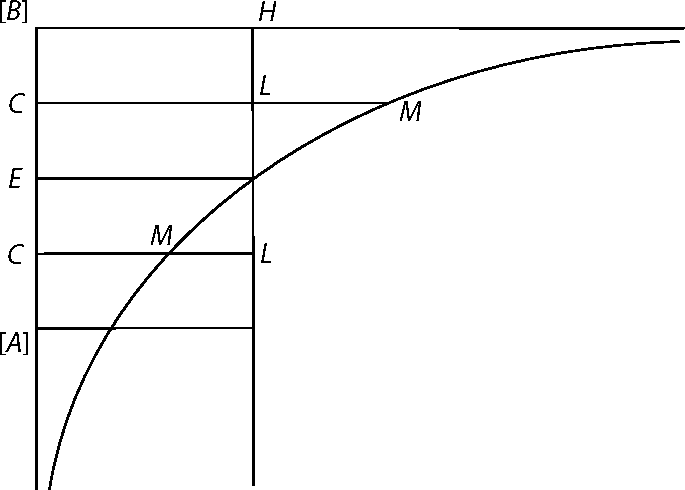
\includegraphics[width=0.45\textwidth]{gesamttex/edit_VIII,3/images/LH_37_01_022-023_d4.pdf}}%\\
  \vspace{0.5em}
  \centerline{\normalsize\lbrack\textit{Fig.~4, gestr.}\rbrack}%
 % \vspace{1.5em}% REIN VORLÄUFIG !!!
\normalsize
\count\Bfootins=1000
\count\Afootins=1200
\count\Cfootins=1200
\newpage
\pstart
\noindent
Angulo ad $AB$
\edtext{recto, ducatur}{%
\lemma{recto,}\Bfootnote{%
\textit{(1)}~ducta
\textit{(2)}~ducatur%
~\textit{L}}}
$A,$ et compleatur rectangulum\protect\index{Sachverzeichnis}{rectangulum} $GABH,$ ac
\edtext{centro $G,$ et asymptotis\protect\index{Sachverzeichnis}{asymptotos}}{%
\lemma{centro}\Bfootnote{%
\hspace{-0,5mm}$G,$
\textbar~et \textit{erg.}~%
\textbar\ asymptotis%
~\textit{L}}}
\hspace{0,1mm}$GA,$ \hspace{0,1mm}$GH,$\hspace{0,1mm}
\edtext{describatur\hspace{0,1mm} ad\hspace{0,1mm} partes\hspace{0,1mm} $B$ Hyperbola\protect\index{Sachverzeichnis}{hyperbola}}{%
\lemma{describatur}\Bfootnote{%
\hspace{-0,5mm}\textbar~%
\textit{(1)}~ad $KN$
\textit{(2)}~ad partes $B$
\textit{erg.}~%
\textbar\ Hyperbola%
~\textit{L}}}
$KMMN,$ talis,
ut ex $M$ ducta
\edtext{utcunque}{%
\lemma{utcunque}\Bfootnote{\textit{erg.~L}}}
ordinata\protect\index{Sachverzeichnis}{ordinata} normali $ML$ in $GH,$
sit rectangulum $GLM,$ semper aequale ipsi $ae$
seu rectangulo\protect\index{Sachverzeichnis}{rectangulum} $GE$ sub $GA$ sive $a,$
et $AE$ sive $e.$
(\phantom)\hspace*{-1.2mm}%
Unde si $a$ et $e$ sumantur aequales erit $E$ vertex Hyperbolae.\protect\index{Sachverzeichnis}{hyperbola}%
\phantom(\hspace*{-1.2mm})
Ex hac constructione\protect\index{Sachverzeichnis}{constructio}
\edtext{patet $LM$ esse $\displaystyle ae : x$ et $CL$ esse $a.$}{%
\lemma{patet}\Bfootnote{%
\textit{(1)}~esse $LM$ =\
\textit{(2)}~$LM$ esse $\displaystyle ae : x$ et
\textbar~et \textit{streicht Hrsg.}~%
\textbar\ $CL$ esse $a.$%
~\textit{L}}}
Ergo $CM$ est
\edtext{$\displaystyle a - ae : x,$
et potentia\protect\index{Sachverzeichnis}{potentia acquisita}
a pondere $C$ descendente\protect\index{Sachverzeichnis}{pondus descendens} acquisita}{%
\lemma{$\displaystyle a - ae : x,$}\Bfootnote{%
\textit{(1)}~et velocitas acquisita\protect\index{Sachverzeichnis}{velocitas acquisita}
\textit{(2)}~et potentia a pondere $C$ descendente
\textit{(a)}~acquisita
\textit{(b)}~acquisita%
~\textit{L}}}
in loco quovis $C,$
\edtext{erit repraesentata}{%
\lemma{erit}\Bfootnote{%
\textit{(1)}~aequalis
\textit{(2)}~repraesentata%
~\textit{L}}}
spatio Hyperbolico $KBCMK.$\protect\index{Sachverzeichnis}{spatium hyperbolicum}
Et
\edtext{summa potentia}{%
\lemma{summa}\Bfootnote{%
\textit{(1)}~velocitas\protect\index{Sachverzeichnis}{velocitas acquisita}
\textit{(2)}~potentia%
~\textit{L}}}
acquisita\protect\index{Sachverzeichnis}{potentia acquisita} in
\edtext{puncto $E,$ repraesentabitur}{%
\lemma{puncto}\Bfootnote{%
\hspace{-0,5mm}$E,$
\textit{(1)}~aequabitur
\textit{(2)}~repraesentabitur%
~\textit{L}}}
trilineo Hyperbolico $KBEK.$\protect\index{Sachverzeichnis}{trilineum hyperbolicum}
Nam Hyperbola\protect\index{Sachverzeichnis}{hyperbola} rectam $AB$ secat in $E.$
Sed % \protect\index{Sachverzeichnis}{gradus potentiae}
\edtext{gradus 
% \lbrack potentiae\rbrack\ 
post $E,$}{%
\lemma{gradus}\Bfootnote{%
\hspace{-0,5mm}\textbar~velocitatis\protect\index{Sachverzeichnis}{gradus velocitatis} \textit{gestr.}~%
% \textbar\ potentiae \textit{erg. Hrsg.}~%
\textbar\ post $E,$%
~\textit{L}}}
qui cadunt in alteram partem ipsius rectae $AB$\lbrack,\rbrack\
non sunt acquisitiones sed
\edtext{detractiones
quia quod detrahitur majus est, quam quod additur.
Ergo descendet pondus\protect\index{Sachverzeichnis}{pondus descendens}
eousque, donec ut}{%
\lemma{detractiones}\Bfootnote{%
\textit{(1)}~. Eousque
\textit{(2)}~quia quod \lbrack...\rbrack\ quam quod
\textit{(a)}~accedit
\textit{(b)}~additur. Ergo descendet pondus eousque, 
\textit{(aa)}~ut
\textit{(bb)}~donec ut%
~\textit{L}}}
in $F$
\edtext{sit $NFEN = KBEK$}{%
\lemma{sit}\Bfootnote{%
\textit{(1)}~$EFNE = KF$
\textit{(2)}~$NFEN = KBEK$%
~\textit{L}}}
seu $KBFNEK$
(\phantom)\hspace*{-1.2mm}%
id est $KBEK - NFEN$%
\phantom(\hspace*{-1.2mm})
$=$ Nihilo.\protect\index{Sachverzeichnis}{nihilum}
Quod est notandum%
\edtext{}{\lemma{\textit{Am Rand:}}\Afootnote{NB}}
ut appareat quomodo in figuris\protect\index{Sachverzeichnis}{figura}
destructio\protect\index{Sachverzeichnis}{destructio} seu nihilum\protect\index{Sachverzeichnis}{nihilum} exhibeatur.
Jam investigandum 
%est
%\edtext{punctum $F.$
%% % % % % % % % % %
%\edlabel{LH_37_01_023r_punctumF_1}%
%Est autem punctum $F$ tale\lbrack,\rbrack\
%seu recta $AF = x$ talis\lbrack,\rbrack\
%ut sit
%$\displaystyle\!\int\!\overline{a\, d\overline{x}\protect\vphantom{\overline{ae : x}\,dx}}
%\,=
%\lbrack\!\!\int\!\overline{\overline{ae : x}\,dx}\rbrack$
%% \edtext{}{%
%% \lemma{$\!\!\int\!\overline{ae : x}\, dx$}%
%% \Bfootnote{\textit{L~ändert Hrsg.}}} %%## %%##
%seu ut sit rectangulum $FH$\protect\index{Sachverzeichnis}{rectangulum}%
%~= quadrilineo\protect\index{Sachverzeichnis}{quadrilineum hyperbolicum}
%\lbrack$KHRNK$\rbrack.
%\edlabel{LH_37_01_023r_punctumF_2}%
%% % % % % % % % % %
%Constat vero}{%
%\lemma{punctum}\Bfootnote{%
%\hspace{-0,5mm}$F$
%\textit{(1)}~, constat enim
%\textit{(2)}~. Est autem \lbrack...\rbrack\ ut sit
%\textbar~$\displaystyle\!\!\int\!\overline{ae : x}\, dx$ \textit{ändert Hrsg.}~%
%\textbar\ seu ut sit rectangulum $FH$~= quadrilineo
%\textbar~$KHFMK$ \textit{ändert Hrsg.}~%
%\textbar~. Constat vero%
%~\textit{L}}}
\edtext{est punctum $F.$
% % % % % % % % % %
\edlabel{LH_37_01_023r_punctumF_1}%
Est autem punctum $F$ tale\lbrack,\rbrack\
seu recta $AF = x$ talis\lbrack,\rbrack\
ut sit
$\displaystyle\!\!\!\int\!\overline{a\, d\overline{x}\protect\vphantom{\overline{ae : x}\,dx}}
\,=
\lbrack\!\!\int\!\overline{\overline{ae : x}\,dx}\rbrack$
seu ut sit rectangulum $FH$\protect\index{Sachverzeichnis}{rectangulum}%
~= quadrilineo\protect\index{Sachverzeichnis}{quadrilineum hyperbolicum}
\lbrack$KHRNK$\rbrack.
\edlabel{LH_37_01_023r_punctumF_2}%
% % % % % % % % % %
Constat vero}{%
\lemma{est}\Bfootnote{%
\hspace{-0,5mm}punctum $F$
\textit{(1)}~, constat enim
\textit{(2)}~. Est autem \lbrack...\rbrack\ sit $\displaystyle\!\!\!\int\!\overline{a\, d\overline{x}\protect\vphantom{\overline{ae : x}\,dx}}\,=$
\textbar~$\displaystyle\!\!\int\!\overline{ae : x}\, dx$ \textit{ändert Hrsg.}~%
\textbar\ seu ut \lbrack...\rbrack\ $FH$~= quadrilineo % sit rectangulum 
\textbar~$KHFMK$ \textit{ändert Hrsg.}~%
\textbar~. Constat vero%
~\textit{L}}}
esse
\edtext{spatia}{%
\lemma{spatia}\Bfootnote{\textit{erg.~L}}}
$KHLMK$ progressionis arithmeticae,\protect\index{Sachverzeichnis}{progressio arithmetica}
si
\edtext{rectae}{%
\lemma{rectae}\Bfootnote{\textit{erg.~L}}}
$GL$ vel $AC$ sint progressionis Geometricae,\protect\index{Sachverzeichnis}{progressio geometrica}
\edtext{seu si spatia illa ut numeri, rectas has esse ut logarithmos,\protect\index{Sachverzeichnis}{logarithmus}}{%
\lemma{seu}\Bfootnote{%
\hspace{-0,5mm}si
\textit{(1)}~illi ut numeri, hos esse ut L
\textit{(2)}~spatia illa \lbrack...\rbrack\ ut logarithmos,%
~\textit{L}}}
\edtext{ergo si}{%
\lemma{ergo}\Bfootnote{%
\textit{(1)}~fiet
\textit{(2)}~si%
~\textit{L}}}
$GH$ sit $h$ vel unitas,\protect\index{Sachverzeichnis}{unitas}
cujus logarithmus\protect\index{Sachverzeichnis}{logarithmus} est 0,
sitque $AE,$ $e,$ $\displaystyle\frac{AC}{AB},$ vel
\edtext{$\displaystyle\frac{\lbrack GL\rbrack}{AB}$}{%
\lemma{$GH$}\Bfootnote{\textit{L~ändert Hrsg.}}}
\edtext{sit $\displaystyle \overline{e : h}^{\boxed{\scriptstyle{v : h}}} \!= x : h$ erunt}{%
\lemma{sit}\Bfootnote{%
\textit{(1)}~$\displaystyle ev : h = x$
\textit{(2)}~$\displaystyle \overline{e : h}^{\protect\boxed{\scriptstyle{v : h}}} \!= x : h$
\textit{(a)}~erit
\textit{(b)}~erunt%
~\textit{L}}}
spatia $KHLMK,$\protect\index{Sachverzeichnis}{spatium hyperbolicum}
ut \edtext{$v % \,\overline{AB} 
= qv % \,\overline{AB}
$\lbrack,\rbrack\
\lbrack$KHPEK$\rbrack\ erit ut $\log e,$
% \edtext{}{%
% \lemma{$\log e$}\Cfootnote{%
% Das Logarithmuszeichen ist zuweilen mit Punkt ($\log.$), zuweilen ohne Punkt ($\log$) geschrieben.
% Die Form ohne Punkt wird hier einheitlich verwendet.}}
et $KHRNK$ ut $\log x$\lbrack,\rbrack\
posito $AF,\ x,$}{%
\lemma{$v = qv$}\Bfootnote{%
% \hspace*{-0,5mm}%
% \textbar~$\overline{AB}$ \textit{erg.}~%
% \textbar\ $=\ qv$
% \textbar~$\overline{AB}$ \textit{erg.}~%
% \textbar\
\textit{(1)}~et debet esse $a$
\textit{(2)}~Et debet esse $e\ -$
\textit{(3)}~\textbar~$KHFEK$ \textit{ändert Hrsg.}~%
\textbar\ erit ut \lbrack...\rbrack\ posito $AF,\ x,$%
~\textit{L}}}
ex natura logarithmorum,\protect\index{Sachverzeichnis}{natura logarithmi}
\edtext{fiet $\displaystyle \overline{v : h} \cdot \log e = \log x.$}{%
\lemma{fiet}\Bfootnote{%
\textit{(1)}~$e : h$
\textit{(2)}~$\displaystyle \overline{v : h} \cdot \log e = \log x.$%
~\textit{L}}}
Nam $\log h$
\edtext{est $=\ 0.$ Ergo}{%
\lemma{est}\Bfootnote{%
\hspace{-0,5mm}$=\ 0.$
\textit{(1)}~Jam
\textit{(2)}~Ergo%
~\textit{L}}}
$v = h \cdot \log x : \log e$
et $KHLMK = qh \cdot \log x : \log e.$
Ergo in casu quo $x = e$
fit
\edtext{\lbrack $KHPEK\rbrack}{%
\lemma{$KLPEK$}\Bfootnote{\textit{L~ändert Hrsg.}}}
= qh$
\edtext{\lbrack quam}{%
\lemma{\lbrack quam}\Cfootnote{Eckige Klammer von Leibniz.}}
quantitatem detrahendo a rectangulo $PB$,\protect\index{Sachverzeichnis}{rectangulum}
seu ab $a \cdot \overline{h - e},$
fit $ah - ae - qh = KBEK.$
Sit jam $AF = x,$
erit
$\edtext{\lbrack EPRNE\rbrack}{%
\lemma{$EPRNP$}\Bfootnote{\textit{L~ändert Hrsg.}}}
= qh \cdot \log x : \log e - qh,$
unde auferendo $PF,$ seu $a\, \overline{e - x},$
fiet $qh \cdot \log x : \log P\, \ovalbox{$-\ qh - ae$} + ax = NFEN = KBEK = ah\, \ovalbox{$-\ ae - qh$}$
seu $qh \cdot \log x : \log e = a \cdot \overline{h - x};$
quae aequatio\protect\index{Sachverzeichnis}{aequatio} determinat punctum $x$
quod etiam inveniri potest per intersectionem rectae et lineae logarithmicae.\protect\index{Sachverzeichnis}{linea logarithmica}%
\edtext{}{% ACHTUNG GETRIXT !!!!!!!!!
\lemma{\hspace*{1,7mm}\textit{Neben} \lbrack\textit{Fig.~5}\rbrack:}\killnumber%
\Afootnote{%
\quad $BH,\ a.$
\quad $AB,\ 2e.$
\quad $BK = a : 2.$
\quad $A\scriptstyle\textit{1}\displaystyle C\ \overline{3 : 2}\, e.$
\quad $\scriptstyle\textit{1}\displaystyle C \scriptstyle\textit{1}\displaystyle L = 2a : 3.$%
%\newline%
}}%
\pend
\vspace{2.0em}%% REIN VORLÄUFIG !!!
  \centerline{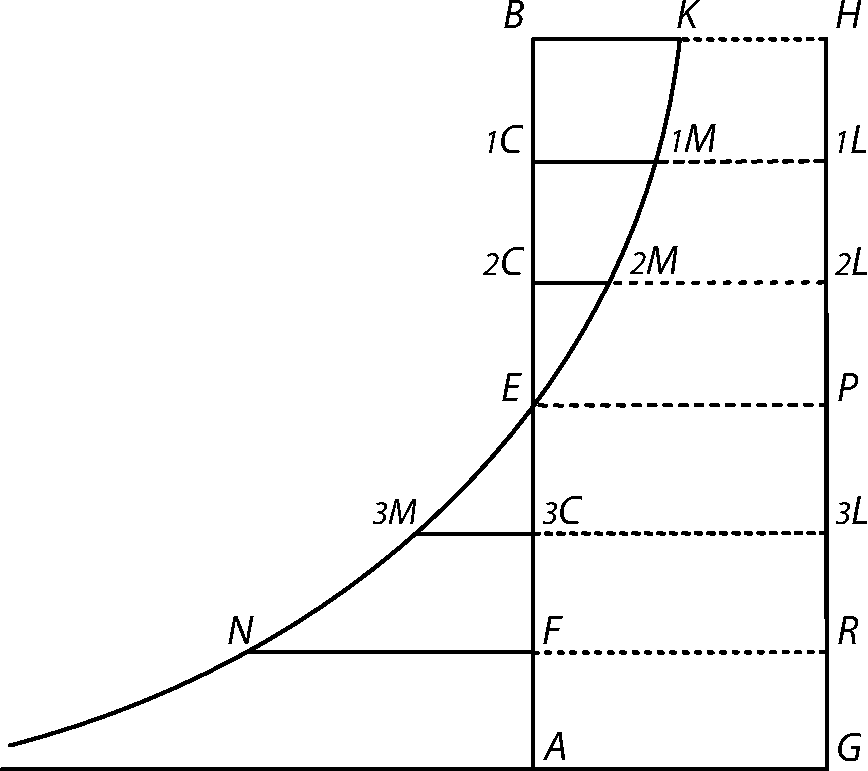
\includegraphics[width=0.58\textwidth]{gesamttex/edit_VIII,3/images/LH_37_01_022-023_d5.pdf}}%
  \label{LH_37_01_023r_fig.5}%
  \vspace{0.5em}
  \centerline{\normalsize\lbrack\textit{Fig.~5}\rbrack}%
  \newpage% REIN VORLÄUFIG !!!
%\vspace{0.5em}
\pstart%
\noindent%
%
\lbrack\textit{Nachfolgend kleingedruckter Text in L gestrichen:}\rbrack
\pend%
\vspace*{0.5em}
\footnotesize%
\pstart%
\noindent%
Seu etiam sic:
$\displaystyle x^{\frac{qh}{\cdot}} \!\!=\ e^{\frac{a\, \overline{h - x}}{\cdot}}$
quod si ponamus $a = q$
\edtext{fiet:}{%
\lemma{\textit{Über dem Wort} \footnotesize{fiet} \normalsize\textit{ebenfalls gestrichen:}}%
\Afootnote{\footnotesize{Imo non fiet.}\vspace{-4mm}}}
\edtext{$\displaystyle x^h \!= \, e^{h - x},$
seu ponentes $h = 1$ fit $\displaystyle x^{\frac{1 : \overline{1 - x}}{\cdot}} \!\!= \, e$
}{%
\lemma{$\displaystyle x^h \!= \, e^{h - x},$}\Bfootnote{%
\textit{(1)}~seu $\displaystyle x^{1 : h - %\phantom{h}
}$%\hspace*{-2mm}
\textit{(2)}~seu ponentes $h = 1$ fit $\displaystyle x^{\frac{1 : \overline{1 - x}}{\cdot}} \!\!= \, e$%
~\textit{L}
}}
eritque
\edtext{$x = AF.$
Hinc si $x$ sit 1 erit}{%
\lemma{$x = AF.$}\Bfootnote{%
\textit{(1)}~Seu sit $a$
\textit{(2)}~Hinc si $x$ sit
\textit{(a)}~$\displaystyle\frac{1}{2}$ erit
\textit{(b)}~1 erit%
~\textit{L}}}
$e\ =$ infinite parvae.
Si sit $\displaystyle x = \frac{1}{2}$ fiet $\displaystyle e = \frac{1}{2}\protect\boxed{\displaystyle 2} = \frac{1}{4}.$
% % Ende footnotesize.
% \edtext{}{%
% \lemma{logarithmicae.}\Bfootnote{%
% \hspace*{-0,5mm}\textbar~Seu etiam sic:
% $\displaystyle x^{\frac{qh}{\cdot}} \!\!=\ e^{\frac{a\, \overline{h - x}}{\cdot}}$
% quod si ponamus $a = q$ fiet: ((HIER AFOONOTE))
% $\displaystyle x^h = e^{h - x},$
%%% \textit{(1)}~seu $\displaystyle x^{1 : h - \phantom{h}}$
%%% \textit{(2)}~seu ponentes $h = 1$ fit $\displaystyle x^{\frac{1 : \overline{1 - x}}{\cdot}} = e$ eritque $x = AF.$
%%% \textit{(a)}~Seu sit $a$
%%% \textit{(b)}~Hinc si $x$ sit
%%% \textit{(aa)}~$\displaystyle\frac{1}{2}$ erit
%%% \textit{(bb)}~1 erit $e\ =$ infinite parvae. Si sit $\displaystyle x = \frac{1}{2}$ fiet $\displaystyle e = \frac{1}{2}\protect\boxed{2} = \frac{1}{4}.$
% \textit{gestr.}~%
% \textbar\ Idem
% ~\textit{L}}}
\pend%%
\count\Bfootins=1200
\count\Afootins=1200
\count\Cfootins=1200
\vspace{0.5em}%
\normalsize%
\pstart%
\noindent%
Idem etiam brevius sic
\edtext{invenitur.\rbrack}{%
\lemma{invenitur.\rbrack}\Cfootnote{%
Eckige Klammer von Leibniz.}}
Inventum est
\edtext{supra}{%
\lemma{supra}%
\Cfootnote{S.~\refpassage{LH_37_01_023r_punctumF_1}{LH_37_01_023r_punctumF_2}.}}
in casu puncti $F$ quaesiti esse rectang. $FH$\protect\index{Sachverzeichnis}{rectangulum}
aequale spatio quadrilineo hyperbolico $KHRNK,$%
\protect\index{Sachverzeichnis}{spatium hyperbolicum}\protect\index{Sachverzeichnis}{quadrilineum hyperbolicum}
seu rectang. $FH$\protect\index{Sachverzeichnis}{rectangulum} est $\displaystyle a \cdot \overline{h - x}$
et quadrilin. $KHRNK$ est ad qua\-drlin.\protect\index{Sachverzeichnis}{quadrilineum hyperbolicum}
\edtext{$KHPEK,$ seu ad $qh,$ ut $\log AF$ seu}{%
\lemma{$KHPEK,$}\Bfootnote{%
\textit{(1)}~ut $\log AF$ seu
\textit{(2)}~seu ad $qh,$ ut $\log AF$ seu%
~\textit{L}}}
$\log x$ ad $\log e.$
Ergo fit $qv = a \cdot \overline{h - x} = qh \cdot \log x : \log e.$
Prorsus ut
\edtext{antea.
%
\lbrack23~v\textsuperscript{o}\rbrack\ % Blatt 23v
%
Etsi autem $a$ assumserimus pro arbitrio,\protect\index{Sachverzeichnis}{arbitrium}}{%
\lemma{antea.}\Bfootnote{%
\textit{(1)}~Jam quia \lbrack23~v\textsuperscript{o}\rbrack\ $a$ assumsimus pro arbitrio
\textit{(2)}~Etsi autem \lbrack...\rbrack\ pro arbitrio,%
~\textit{L}}}
tamen ab eo semel assumto, certo modo pendet $q.$
Et non licet facere $q = a,$
nam fieret $qh = ah,$ seu quadrilin. $KHPEK$
(\phantom)\hspace*{-1.2mm}%
quod fecimus $qh$%
\phantom(\hspace*{-1.2mm})
erit aeq. rectangulo $BG$\protect\index{Sachverzeichnis}{rectangulum}
(\phantom)\hspace*{-1.2mm}%
seu $ah$%
\phantom(\hspace*{-1.2mm}),
pars toti\lbrack;\rbrack\
quod est absurdum.
Porro aequationem Logarithmicam\protect\index{Sachverzeichnis}{aequatio logarithmica}
mutando in potentialem\protect\index{Sachverzeichnis}{aequatio potentialis}\lbrack,\rbrack\
quia habuimus $\displaystyle \log e = \log x \cdot qh : a\,\overline{a - x},$
fiet inde $\displaystyle e = x^{\,\boxed{\scriptstyle qh : \overline{a \cdot \overline{a - x}}}}\displaystyle.$
\pend%
%
%
\pstart%
\edtext{\lbrack Etsi}{%
\lemma{\lbrack Etsi}\Cfootnote{%
Eckige Klammer von Leibniz.}}
autem $q$ sit semper minor quam $a,$
videamus tamen an non mutata $a,$
mutetur ratio inter $a$ et $q,$
et an non proinde reperiri possit ratio omnium possibilium minima,\protect\index{Sachverzeichnis}{ratio minima}
ubi $q$ maxime % \edtext{}{%
% \lemma{ubi}\Bfootnote{%
% \textit{(1)}~$q$ ma
% \textit{(2)}~$q$ maxime%
% ~\textit{L}}}
vicina ipsi $a.$
Sed video nihil hinc duci,
semperque eandem manere proportionem inter $q$ et $a.$
Nam
\edtext{sit $EC,$}{%
\lemma{sit}\Bfootnote{%
\textit{(1)}~$AE$
\textit{(2)}~$EC,$
\textit{(3)}~$EC,$%
~\textit{L}}}
$y,$
\edtext{fiet $KHPEK$}{%
\lemma{fiet}\Bfootnote{%
\textit{(1)}~$KHPMK$
\textit{(2)}~$KHPEK$%
~\textit{L}}}
aeq. $\displaystyle \!\!\!\int\!\!\overline{ae : \overline{e + x},\ d\overline{x} = qh}$
et ista
\edtext{summa dividens $ah,$}{%
\lemma{summa}\Bfootnote{%
\textit{(1)}~divisa per $a$
\textit{(2)}~dividens
\textit{(a)}~$ae,$
\textit{(b)}~$ah,$%
~\textit{L}}}
dabit rationem inter $ah$ et $qh,$
seu inter $a$ et $q,$
quam faciendo omnium possibilium minimam $\mu,$\protect\index{Sachverzeichnis}{ratio minima}
fiet $\displaystyle \cancel{a}e\!\!\!\int\!\!\overline{1 : \overline{e + x}, d\overline{x}} : \cancel{a}h = \mu,$
ubi patet
\edtext{evanescere $a,$}{%
\lemma{evanescere}\Bfootnote{%
\textit{(1)}~$h$
\textit{(2)}~$a,$%
~\textit{L}}}
adeoque non posse hinc inveniri valorem\protect\index{Sachverzeichnis}{valor}
\edtext{ipsius $h.$\rbrack}{%
\lemma{ipsius $h.$\rbrack}\Cfootnote{%
Eckige Klammer von Leibniz.}}
\pend%
%
%
\pstart%
Illud\edlabel{LH_37_01_023v_Schluss_girt-1}
potius consideratione dignum videtur,
ex calculo\protect\index{Sachverzeichnis}{calculus} % \edtext{}{%
% \lemma{videtur,}\Bfootnote{%
% \textit{(1)}~ex c
% \textit{(2)}~ex calculo%
% ~\textit{L}}}
nostro duci modum aestimandi
ex quanta altitudine\protect\index{Sachverzeichnis}{altitudo lapsus} cadere debeat
\edtext{pondus\protect\index{Sachverzeichnis}{pondus cadens} datum,
ut aerem comprimat\protect\index{Sachverzeichnis}{aer compressus} intra datum}{%
\lemma{pondus}\Bfootnote{%
\hspace{-0,5mm}datum,
\textit{(1)}~ut ad da
\textit{(2)}~ut aerem comprimat intra datum%
~\textit{L}}}
spatium;
seu quousque aer\protect\index{Sachverzeichnis}{aer compressus}
datae compressionis\protect\index{Sachverzeichnis}{compressio}
\edtext{pondus\protect\index{Sachverzeichnis}{pondus cadens} datum}{%
\lemma{pondus}\Bfootnote{%
\textit{(1)}~data
\textit{(2)}~datum%
~\textit{L}}}
attollere possit,
seu quanta sit vis compressionis\protect\index{Sachverzeichnis}{vis compressionis} viva\protect\index{Sachverzeichnis}{vis viva}
\edtext{respectu dati}{%
\lemma{respectu}\Bfootnote{% \hspace*{-0,5mm}
\textbar~corporis \textit{gestr.}~%
\textbar\ dati%
~\textit{L}}}
ponderis.
Nam pondus\protect\index{Sachverzeichnis}{pondus cadens}
\edtext{quod cum}{%
\lemma{quod}\Bfootnote{%
\textit{(1)}~super
\textit{(2)}~cum%
~\textit{L}}}
aere intra $AE$ compresso\protect\index{Sachverzeichnis}{aer compressus}
in aequilibrio\protect\index{Sachverzeichnis}{aequilibrium} est,
cadens ex altitudine $BF$\protect\index{Sachverzeichnis}{altitudo lapsus} aerem
\edtext{dictum, diffusum\protect\index{Sachverzeichnis}{aer diffusus} per $AB$}{%
\lemma{dictum,}\Bfootnote{%
\hspace{-0,5mm}diffusum per $AB$
\textit{erg.~L}}}
comprimet
% intra $AF.$%
%\edlabel{LH_37_01_023v_Schluss_girt-2}
%\pend%
%\vspace*{0.5em}
%%
%\pstart%
%\noindent%
%\lbrack\textit{Nachfolgend kleingedruckter Text in L gestrichen:}\rbrack
%\pend%
%\vspace*{0.5em}
%\footnotesize%
%\pstart%
%\noindent%
%Dato igitur pondere\protect\index{Sachverzeichnis}{pondus cadens} adeoque data $AE$
%intra quam compressus aer\protect\index{Sachverzeichnis}{aer compressus}
%dati voluminis,\protect\index{Sachverzeichnis}{volumen}
%cum pondere\protect\index{Sachverzeichnis}{pondus cadens} dato in
%\edtext{aequilibrio\protect\index{Sachverzeichnis}{aequilibrium} foret,
%dataque $AF$ intra quam aer idem revera est compressus,\protect\index{Sachverzeichnis}{aer compressus}
%dabitur}{%
%\lemma{aequilibrio}\Bfootnote{%
%\textit{(1)}~est,
%\textit{(2)}~foret,
%\textit{(a)}~dabitur per
%\textit{(b)}~et data altitudine casus $BF,$ dabitur
%\textit{(c)}~dataque $AF$ \lbrack...\rbrack\ compressus, dabitur%
%~\textit{L}}}
%$AB$ ad
%\edtext{quem
%\lbrack\textit{Satz bricht ab.}\rbrack\
%Nam}{%
%\lemma{quem}\Bfootnote{%
%\textit{(1)}~Verum quando
%\textit{(2)}~Nam%
%~\textit{L}}}
%pondus aequilibratum aeri compresso\protect\index{Sachverzeichnis}{aer compressus}
%\edtext{intra $AE,$ cadere incipiens\protect\index{Sachverzeichnis}{pondus cadens}}{%
%\lemma{intra}\Bfootnote{%
%\hspace{-0,5mm}$AE,$
%\textit{(1)}~cadens
%\textit{(2)}~cadere incipiens%
%~\textit{L}}}
%in eundem aerem\protect\index{Sachverzeichnis}{aer compressus}
%\edtext{(\phantom)\hspace*{-1.2mm}%
%quadrato velocitatis\protect\index{Sachverzeichnis}{quadratum velocitatis} seu%
%\phantom(\hspace*{-1.2mm})}{%
%\lemma{(\phantom)\hspace*{-1.2mm}quadrato}\Bfootnote{%
%\hspace{-0,5mm}velocitatis seu\phantom(\hspace*{-1.2mm})
%\textit{erg.~L}}}
%potentia\protect\index{Sachverzeichnis}{potentia} quae sit ut $KBEK$
%comprimet eundem aerem\protect\index{Sachverzeichnis}{aer compressus} ex $AE$ in $AF.$
%Sed quomodo
%\edtext{inveniemus $EB$ altitudinem}{%
%\lemma{inveniemus}\Bfootnote{%
%\textbar~$AB$ seu \textit{gestr.}~%
%\textbar\ $EB$ altitudinem%
%~\textit{L}}}
%\edtext{lapsus.\protect\index{Sachverzeichnis}{altitudo lapsus}
%Data velocitate\protect\index{Sachverzeichnis}{velocitas acquisita}
%vel potentia\protect\index{Sachverzeichnis}{potentia acquisita} datur}{%
%\lemma{lapsus.}\Bfootnote{%
%\textit{(1)}~In eo est difficultas, quod
%\textit{(2)}~Data velocitate 
%\textit{(a)}~datur
%\textit{(b)}~vel potentia datur%
%~\textit{L}}}
%altitudo\protect\index{Sachverzeichnis}{altitudo lapsus} ex qua acquisita est, 
%adeoque
%\edtext{data $\displaystyle\frac{1}{2}vv,$
%datur $\displaystyle \!\int\! \overline{e - \overline{e : x}, d\overline{x}},$}{%
%\lemma{data}\Bfootnote{%
%\hspace{-0,5mm}$\displaystyle\frac{1}{2}vv,$
%\textit{(1)}~seu
%\textit{(2)}~datur
%\textit{(a)}~$\displaystyle\frac{1}{2}$
%\textit{(b)}~$\displaystyle \!\int\! \overline{e - \overline{e : x}, d\overline{x}},$%
%~\textit{L}}}
%ex qua data etiam datur $x.$
\edtext{}{%
{\xxref{LH_37_01_023v_gestrichen_kglhdubl-1}{LH_37_01_023v_gestrichen_kglhdubl-2}}%
{\lemma{intra}\Bfootnote{%
\hspace*{-0,5mm}$AF.$
\textit{(1)}~Dato igitur pondere adeoque data $AE$
intra quam compressus aer\protect\index{Sachverzeichnis}{aer compressus}
dati voluminis,\protect\index{Sachverzeichnis}{volumen}
cum pondere\protect\index{Sachverzeichnis}{pondus cadens} dato in
aequilibrio\protect\index{Sachverzeichnis}{aequilibrium}
\textit{(a)}~est,
\textit{(b)}~foret,
\textit{(aa)}~dabitur per
\textit{(bb)}~et data altitudine casus $BF,$ dabitur
\textit{(cc)}~dataque $AF$ intra quam aer idem revera est compressus, dabitur $AB$ ad quem
\textit{(2)}~Verum quando
\textit{(3)}~Nam pondus \lbrack...\rbrack\ intra $AE,$ % aequilibratum aeri compresso
\textit{(a)}~cadens
\textit{(b)}~cadere incipiens in eundem aerem
\textbar~(\phantom)\hspace*{-1.2mm}quadrato velocitatis seu\phantom(\hspace*{-1.2mm}) \textit{erg.}~%
\textbar\ potentia quae \lbrack...\rbrack\ quomodo inveniemus % sit ut $KBEK$ comprimet eundem aerem ex $AE$ in $AF.$ Sed
\textbar~$AB$ seu \textit{gestr.}~%
\textbar\ $EB$ altitudinem lapsus.
\textit{(aa)}~In eo est difficultas, quod
\textit{(bb)}~Data velocitate
\textit{(aaa)}~datur
\textit{(bbb)}~vel potentia \lbrack...\rbrack\ data $\displaystyle\frac{1}{2}vv,$ % datur altitudo ex qua acquisita est, adeoque
\textit{(aaaa)}~seu
\textit{(bbbb)}~datur
\textit{(aaaaa)}~$\displaystyle\frac{1}{2}$
\textit{(bbbbb)}~$\displaystyle \!\int\! \overline{e - \overline{e : x}, d\overline{x}},$ ex \lbrack...\rbrack\ datur $x.$% qua data etiam
~\textit{L}}}}%
\edlabel{LH_37_01_023v_gestrichen_kglhdubl-1}%
intra $AF.$%
\edlabel{LH_37_01_023v_Schluss_girt-2}
\pend%
\vspace*{0.5em}
%
\pstart%
\noindent%
\lbrack\textit{Nachfolgend kleingedruckter Text in L gestrichen:}\rbrack
\pend%
\vspace{0.5em}
\footnotesize%
\pstart%
\noindent%
Nam pondus aequilibratum aeri compresso\protect\index{Sachverzeichnis}{aer compressus}
intra $AE,$ cadere incipiens\protect\index{Sachverzeichnis}{pondus cadens}
in eundem aerem\protect\index{Sachverzeichnis}{aer compressus}
(\phantom)\hspace*{-1.2mm}%
quadrato velocitatis\protect\index{Sachverzeichnis}{quadratum velocitatis} seu%
\phantom(\hspace*{-1.2mm})
potentia\protect\index{Sachverzeichnis}{potentia} quae sit ut $KBEK$
comprimet eundem aerem\protect\index{Sachverzeichnis}{aer compressus} ex $AE$ in $AF.$
Sed quomodo inveniemus $EB$ altitudinem lapsus.\protect\index{Sachverzeichnis}{altitudo lapsus}
Data velocitate\protect\index{Sachverzeichnis}{velocitas acquisita}
vel potentia\protect\index{Sachverzeichnis}{potentia acquisita} datur
altitudo\protect\index{Sachverzeichnis}{altitudo lapsus} ex qua acquisita est,
adeoque data $\displaystyle\frac{1}{2}vv,$
datur $\displaystyle \!\int\! \overline{e - \overline{e : x}, d\overline{x}},$
ex qua data etiam datur $x.$%
\edlabel{LH_37_01_023v_gestrichen_kglhdubl-2}
Quod si pondus cadens\protect\index{Sachverzeichnis}{pondus cadens}
ex altitudine\protect\index{Sachverzeichnis}{altitudo lapsus} quadam
incipiat attingere aerem\protect\index{Sachverzeichnis}{aer compressus}
non aequilibratum sibi sed fortiorem\lbrack,\rbrack\
determinari etiam poterunt omnia Methodo\protect\index{Sachverzeichnis}{methodus} eadem.%
% % Ende Footnotesize.
\pend%
\normalsize
\count\Bfootins=1200
\count\Afootins=1200
\count\Cfootins=1200%
%
%
% ENDE DES STÜCKES auf Blatt 23v in der Mitte (Rest des Blattes leer) 